\documentclass[useAMS,usenatbib]{mn2e}
\pdfminorversion=4

% The following is needed to fix the margins if using Letter-size paper
% REMOVE if your LaTeX uses A4 paper by default
\addtolength\topmargin{-1.8cm}
\usepackage{newtxtext}
\usepackage[varg]{newtxmath}

\usepackage{graphicx}
\usepackage{booktabs}
\usepackage{siunitx}
\bibliographystyle{mn2e}
\usepackage{astrojournals}
\usepackage{fixltx2e}

\begin{document}

\newcounter{ion}
\newcommand\fakesc[1]{\protect\scalebox{1.0}[0.8]{#1}}
\newcommand\ION[2]{\ensuremath{\mathrm{#1\,\fakesc{#2}}}}
\newcommand\ion[2]{\setcounter{ion}{#2}\ION{#1}{\Roman{ion}}}
\newcommand\hii{\ion{H}{2}}
\newcommand\oi{[\ion{O}{1}]}
\newcommand\oiii{[\ion{O}{3}]}
\newcommand\nii{[\ion{N}{2}]}
\newcommand\sii{[\ion{S}{2}]}
\newcommand\siii{[\ion{S}{3}]}
\newcommand\ha{\ensuremath{\mathrm{H\alpha}}}
\newcommand\kms{\ensuremath{\mathrm{km\ s^{-1}}}}
\newcommand\los{\ensuremath{_{\mathrm{los}}}}
\newcommand\pos{\ensuremath{_{\mathrm{pos}}}}
\newcommand\obs{\ensuremath{_{\mathrm{obs}}}}
\newcommand\ins{\ensuremath{_{\mathrm{ins}}}}
\newcommand\rms{\ensuremath{_{\mathrm{rms}}}}
\newcommand\FS{\ensuremath{_{\mathrm{fs}}}}
\newcommand\therm{\ensuremath{_{\mathrm{therm}}}}


\begin{figure}
  \centering
  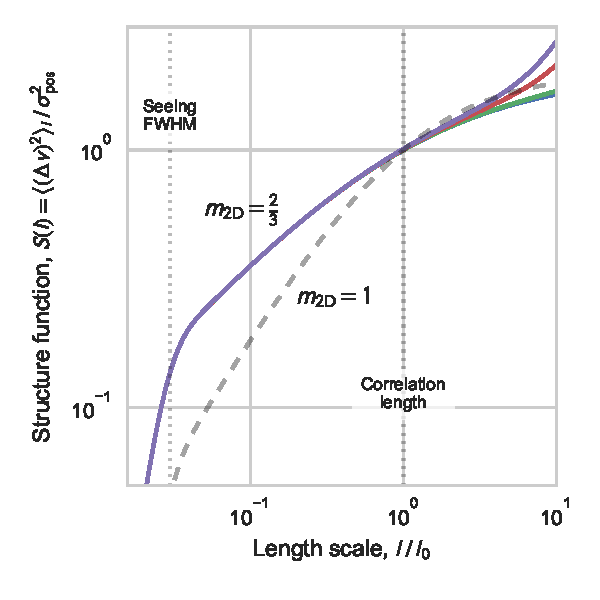
\includegraphics[width=\linewidth]{strucfunc-ideal}
  \caption{Idealized plane-of-sky normalized structure function
    \(S(l) = 2\left[ 1 - C(l) \right]\) for turbulent velocity
    autocovariance of the form
    \(C(l) = 1/\left[1 + (l/l_0)^{m_\mathrm{2D}}\right]\), where
    \(l_0\) is the correlation length of the turbulence. Results for
    Kolmogorov-like turbulence (\(m_\mathrm{2D} = 2/3\)) and a steeper
    spectrum (\(m_\mathrm{2D} = 1\)) are shown.  In the first case,
    different colored lines show the effect of an uncorrected
    linear velocity gradient on the scale of the map (size \(10
    l_0\)), with total amplitude of (top to bottom) 2.0, 1.0, 0.1, and
    0.0 times the turbulent velocity dispersion,
    \(\sigma_\mathrm{pos}\).  At small scales, the effect of seeing
    is shown, assuming a Gaussian FWHM of \(0.03 l_0\). 
  }
  \label{fig:sf-ideal}
\end{figure}

Figure~\ref{fig:sf-ideal} illustrates how various effects modify the
purely turbulent structure functions for a highly idealized case.  The
most promising range of length scales for measuring the turbulent
velocity spectrum is between a few times the seeing width and about
half the correlation length, \(l_0\), of the turbulence.  At scales
larger than \(l_0\), the structure function flattens as it tends
towards the asymptotic value of 2 for a homogeneous random field.  If
there is a linear velocity gradient across the map, then the structure
function will steepen again at the largest scales.  Alternatively, if
the turbulent velocity dispersion is inhomogeneous, being larger in
the center of the map than in the periphery, then the structure
function slope will become negative at the largest scales (not
illustrated).  The figure does not include the effects of noise, but
that is easily dealt with in the case that the noise is ``white''
(spatially uncorrelated, such as shot noise), since the effect is to
simply add a constant value to the structure function at all scales.
This can be estimated either from the variance of velocity differences
at separations significantly less than the seeing width or from
independent observations of the same spatial point, and then
subtracted from the observed structure function prior to analysis.
Spatially correlated ``noise'' due to systematic instrumental effects
is more difficult to deal with, since it will add a spurious
scale-dependent term to the structure function. 


\begin{table}
  \newcommand\C[1]{\multicolumn{1}{c}{#1}}
  \caption{Comparison of structure function slopes}
  \label{tab:sf-lit}
  \centering
  \setlength{\tabcolsep}{0.45em}
  \begin{tabular}{lll@{}r@{\hspace{1.5em}}cl}\toprule
    &     &        & \C{\(\sigma^{2}\)} & \C{Range} & \\
    Reference & Ion & Method & \C{(\kms{})} & \C{(\(''\))} & \C{Slope}\\
    \midrule
    \citealt{ODell:1992a} & \oi{} & Mean & 3:\phantom{0} & 6--85 & \(0.68\):\\
    This paper & \sii{} & Mean & 5.4 & 7--32 & \(0.80 \pm 0.12\)\\
    This paper & \nii{} & Mean & 5.6 & 8--22 & \(0.82 \pm 0.11\)\\
    \citealt{Wen:1993a} & \siii{} & Comp A & 13.8 & 5--20 & \(0.92\):\\
    This paper & \ha{} & Mean & 9.4 & 8--22 & \(1.17 \pm 0.08\)\\
    This paper & \oiii{} & Mean & 10.2 & 8--22 & \(1.18 \pm 0.09\)\\
    \citealt{Castaneda:1988a} & \oiii{} & Comp A & 13.7 & 3--15 & \(0.86 \pm 0.05\)\\
    This paper & \oiii{} & Comp A & 15.3 & 3--15 & \(0.73 \pm 0.05\) \\
    \bottomrule
  \end{tabular}
\end{table}


Previous studies of the velocity structure function in Orion have been
carried out based on slit spectra \citep{Castaneda:1988a, ODell:1992a,
  Wen:1993a}.  Table~\ref{tab:sf-lit} compares these results with our
own for different emission lines, ordered from lower to higher
ionization.  In spite of the differences in methodology, a broad
agreement is seen, with both the magnitude of the velocity dispersion
and the steepness of the structure function slope increasing with
ionization.  The most directly comparable methodology to our own is
that of \citealt{ODell:1992a} who used the flux-weighted mean velocity
of the \oi{} \(\lambda\)6300 line.  The fitted range of \(6''\) to
\(85''\) extends to larger scales than in studies of other lines,
and this biases the slope determination towards lower values due to the
slight curvature of the structure function.    

The other studies are harder to compare with our own since they are
based on multi-component Gaussian fits to the line profiles, such as
shown in Figure~\ref{fig:gauss}.  In order to check the effects of
this methodological difference, we have calculated the \oiii{}
structure function for the strongest component of the three-Gaussian
decomposition of our line profiles (component~A, see
\S\label{sec:plane-sky-versus}), with results that are also included
in Table~\ref{tab:sf-lit}.  We find a slightly larger plane-of-sky
velocity dispersion and shallower structure function than we found
using the mean velocity of the entire profile, which is consistent
with the results of \citet{Castaneda:1988a} for the same line.
Experimentation shows that this is partly due to under-determination
of the Gaussian fits, particularly for components A and B, which are
severely blended at most positions.  This results in a fitting
degeneracy between the velocity separation
\(v_\mathrm{A} - v_\mathrm{B}\) and the flux ratio
\(F_\mathrm{A}/F\mathrm{B}\) of the two components, which spuriously
contributes to the variation in \(v_\mathrm{A}\).  

The structure function slopes obtained by \citet{Mc-Leod:2015b}, based
on integral field spectroscopy with the MUSE instrument
\citep{Weilbacher:2015a} are significantly flatter than all other
studies, and we have decided not to include them in the comparison
table.  For example, they obtain a slope of \(0.29\) for \oiii{} and
\(0.0\) for [\ion{O}{1}].  This appears to be the result of
uncorrected fixed-pattern noise in their mean velocity maps, which can
be seen as tartan-like horizontal and vertical stripes in their
Fig.~10.  We will show in a following paper that once these
instrumental artifacts have been removed, the MUSE results are
consistent with other studies. 



\bibliography{BibdeskLibrary-slavoj}

\end{document}

%%% Local Variables:
%%% mode: latex
%%% TeX-master: t
%%% End:
